\documentclass[a4paper]{article}

\usepackage{INTERSPEECH2018}
\usepackage{cite}

\title{Paper Template for INTERSPEECH 2018}
\name{Dhruv Mishra}
%The maximum number of authors in the author list is twenty. If the number of contributing authors is more than twenty, they should be listed in a footnote or in acknowledgement section, as appropriate.
\address{
  IMS, Uni Stuttgart}
\email{author@university.edu, coauthor@company.com}

\begin{document}

\maketitle
%
\begin{abstract}
  This report describes the paper \cite{dredze2010nlp} which was presented by me and two other papers: \cite{Davis80-COP} and \cite{Davis80-COP}.
\end{abstract}

\section{NLP on spoken documents without ASR}
The paper \cite{dredze2010nlp} describes a technique to apply NLP algorithms directly on spoken documents by transforming the speech data into a vector representation which is very similar to how textual data is represented. The motivation to do is are many:

\begin{itemize}
\item The current popular technique of using an ASR system to transcribe spoken decouments is not very efficient. This method is prone to limitations imposed by the ASR system and error propagation into the entire pipleline.
\item NLP algorithms applied on text data often use simple features like term frequency (tf), inverted document frequency (idf) etc. Requirement for annotations is often very minimal.
\item ASR systems on the other hand require a lot of annotated data, which is not always practical to procure or create.
\end{itemize}

Therefore, a technique to convert speech into an appropriate vector representation which can be used as input to NLP algorithms is presented.

\subsection{Data}
The paper uses a subset of the Switchboard Telephone Speech Corpus. This corpus has 2400 two sided telephone conversations on 70 pre-selected topics. The six most commonly topics were selected: recycling, capital punishment, drug testing, family finance, job benefits, car buying. For these topics, 60 sides of conversations were randomly selected. The resulting data set therefore contained 360 documents spoken by different speakers and was 36 hours in length.

\subsection{Dot Plots}
Dot plots is a method which has been borrowed from bio-informatics. Given character strings s1 and s2, substrings which are common to both of them can be seen as diagonal line segments in the visualisation. If the two strings are same, there will be a main diagonal which will be a result of self similarity. Therefore, search is for line segments other than the main diagonal to identify repetitions.

\subsection{Posteriorgram Representations}
To adapt dot plots for spoken documents, the speech signals must be converted into a sequence of frames. Each frame is represented as the posterior probability distribution over a set of speech sounds given the speech observed at the particular point in time. The paper uses an English phone-set but it claims that it can be used for any language. The reason is that as long as the speech is reliably mapped to a probability distribution over this phone set, different languages will also get mapped into the same domain. This results in the applicability of this representation across different languages, although the paper does not test this hypothesis. This representation is also speaker-independent and provides sparsity to enable efficient storage and computation.

\subsection{Acoustic Dot Plots}
Given a spoken document represented as a sequence of frames represented with posteriorgrams, an acoustic dotplot can be created, similar to the string dot plot where instead of matching characters, the frames are matched instead. This dot plot will have diagonal line segments for frames which are similar.

\subsubsection{Hyperparameters during matching phase}
While matching characters is a simple task, matching frames is not trivial. The paper proposes two parameters to determine what a match is:

\begin{itemize}
\item Kappa: This is the duration of the match in seconds.
\item Tau: The overlap threshold, i.e. the extent of similarity. A value of 1 is an exact match whereas 0.5 means only half of the frame is a match.
\end{itemize}

Decreasing Kappa results in more matched regions and increasing Tau results in less frames getting matched. Both of them increase the number of pseudo-terms.

\subsection{Pseudo Terms}
Pseudo-terms represent a single word or phrase spoken at multiple points throughout the corpus. Each pseudo-term takes the place of a word of phrase in a bag or terms vector space model of a text document and allows the use of standard NLP algorithms. Pseudo-terms are created using by clustering the matched regions in the documents.

\subsubsection{Creating Pseudo-terms}
After finding a set of matched regions, graph clustering is used to aggregate the similar matches into a cluster.
The clusters thus formed are the pseudo-terms which represent a word of a phrase.

To take an example, suppose the phrase “It is sunny today” occurs once in three documents A,B and C. The acoustic dotplots will give three matches: AB, AC and BC. Each of these matches will have slightly different representations since the speakers are different. Using graph clustering, these matches are aggregated into a single cluster. This cluster is a pseudo-term which represents the term “It is sunny today” and has a tf of 3 and idf of 0 (because it occurs in 3 “documents”).

\subsubsection{Evaluation metrics for Clustering}
The clusters created by graph clustering were evaluated on three metrics:

\begin{itemize}
\item Purity: The precision of each cluster, i.e., how many examples in each cluster belong to the same true topic.
Higher values are better.
\item Entropy: how the members of a cluster are distributed amongst the true labels.
Lower values are better.
\item B-cubed: measures clustering effectiveness from the perspective of a user’s inspecting the clustering results.
Higher values are better.
\end{itemize}

\subsubsection{Clustering results}
The pseudo-terms created by graph clustering were compared with two other baseline methods: Phonetic Trigrams (three sequential phones) and Word Transcripts (Unigram, Bigram, Trigram). It must be noted that Word Transcripts is the upper-bound for performance because in the best case, the pseudo-terms created will be the exact representations of words in the textual transcripts.

% add the figure maybe!
Pseudo-terms give perform significantly better than Phonetic Trigrams and almost as good as Word transcripts.


\subsection{Supervised Classification using pseudo-terms}
The pseudo-terms thus created were then used to do a topic classification task, where each document is labelled with the topic it belongs to. The topics were the six most common ones: recycling, capital punishment, drug testing, family finance, job benefits, car buying. Since the labels are balanced, random guessing will yield accuracy of 0.1667. A supervised learning algorithm was trained using labelled data and then asked to label some unseen test data.

The performance evaluated on four popular learning algorithms:MIRA, Confidence Weighted (CW), Maximum Entropy, Support Vector Machines (SVM).

Results:
% add the figure maybe!
Pseudo-terms give perform significantly better than Phonetic Trigrams and almost as good as Word transcripts.


% \begin{figure}[t]
%   \centering
%   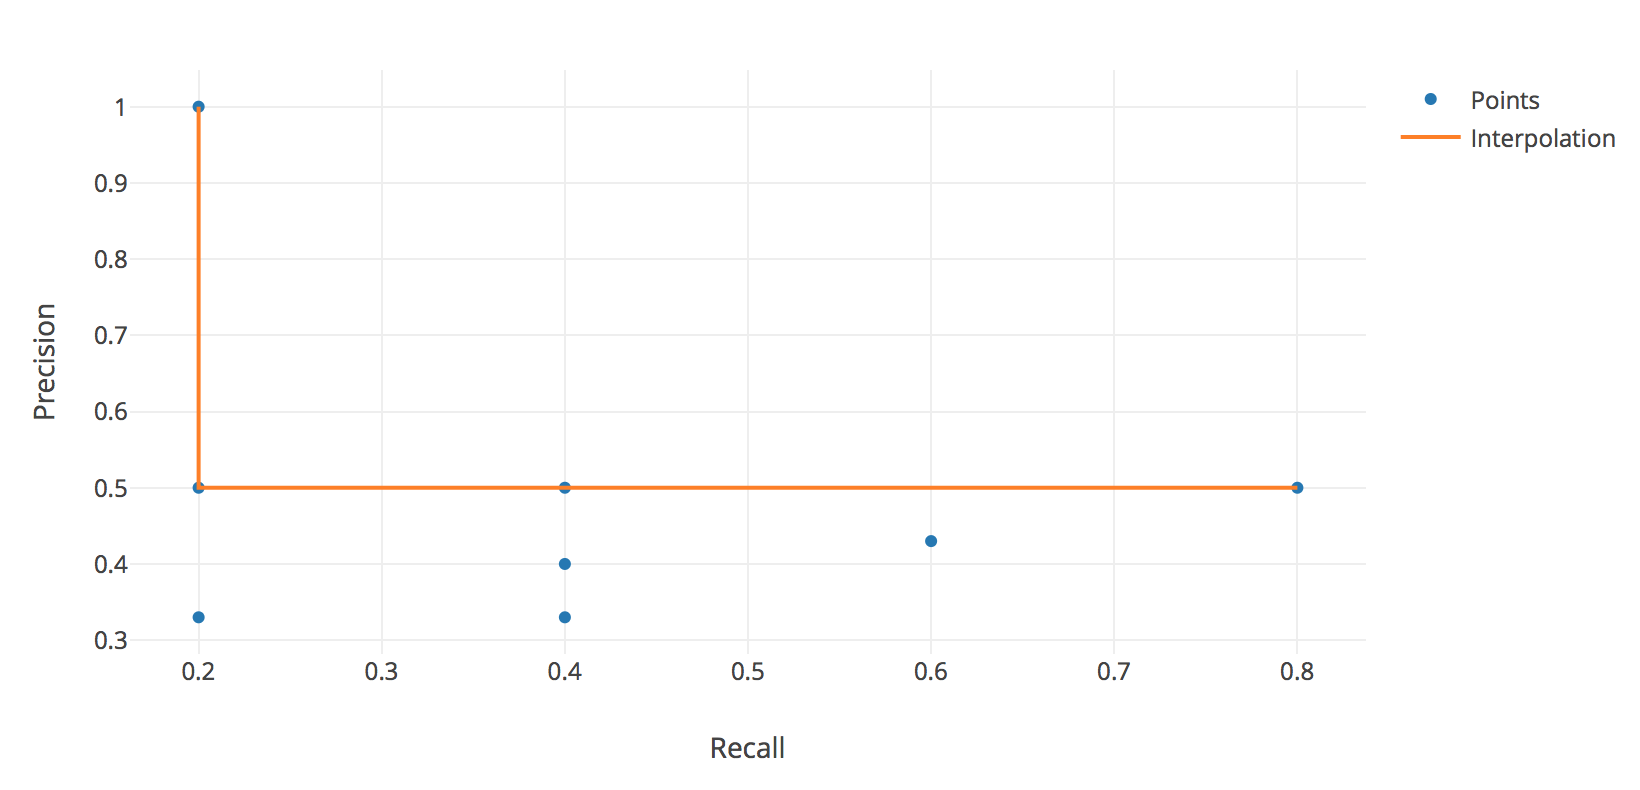
\includegraphics[width=\linewidth]{figure.pdf}
%   \caption{Schematic diagram of speech production.}
%   \label{fig:speech_production}
% \end{figure}

\subsection{Information for Word users only}


\subsection{Hyperlinks}

\subsection{Multimedia files}

The INTERSPEECH organizing committee offers the possibility to submit multimedia files.

\subsection{Page numbering}

Final page numbers will be added later to the document electronically. \emph{Don't make any footers or headers!}


\subsection{References}

The reference format is the standard IEEE one. References should be numbered in order of appearance, for example \cite{Davis80-COP}, \cite{Rabiner89-ATO}, \cite[pp.\ 417--422]{Hastie09-TEO}, and \cite{YourName17-XXX}.

\subsection{Abstract}

\section{Discussion}

This is the discussion. This is the discussion. This is the discussion. Is there any discussion?

\section{Conclusions}
A new strategy to perform unsupervised clustering and supervised classification of spoken documents. The performance is quite close to manual word transcriptions and generally matching or exceeding that achieved with a phonetic recognizer.


\bibliographystyle{IEEEtran}

\bibliography{mybib}

% \begin{thebibliography}{9}
% \bibitem[1]{Davis80-COP}
%   S.\ B.\ Davis and P.\ Mermelstein,
%   ``Comparison of parametric representation for monosyllabic word recognition in continuously spoken sentences,''
%   \textit{IEEE Transactions on Acoustics, Speech and Signal Processing}, vol.~28, no.~4, pp.~357--366, 1980.
% \bibitem[2]{Rabiner89-ATO}
%   L.\ R.\ Rabiner,
%   ``A tutorial on hidden Markov models and selected applications in speech recognition,''
%   \textit{Proceedings of the IEEE}, vol.~77, no.~2, pp.~257-286, 1989.
% \bibitem[3]{Hastie09-TEO}
%   T.\ Hastie, R.\ Tibshirani, and J.\ Friedman,
%   \textit{The Elements of Statistical Learning -- Data Mining, Inference, and Prediction}.
%   New York: Springer, 2009.
% \bibitem[4]{YourName17-XXX}
%   F.\ Lastname1, F.\ Lastname2, and F.\ Lastname3,
%   ``Title of your INTERSPEECH 2018 publication,''
%   in \textit{Interspeech 2018 -- 19\textsuperscript{th} Annual Conference of the International Speech Communication Association, September 2-6, Hyderabad, India Proceedings, Proceedings}, 2018, pp.~100--104.
% \end{thebibliography}

\end{document}
